\subsection{Effects of Parameters}
An important point to note about the models, is that we took the mass to be 120,000kg. However, this mass has been rounded to 2 significant figures, therefore it is important for me to consider the impact it would have on the model if the plane had a mass of 125,000 or a mass of 115,000kg. By taking $m=125,000$ and $m=115000$, and re-solving the 3rd model, I will be able to see the difference it would have on the final equation. 

\input{Model3/ParameterVariation/MassUpperBound.tex}
\begin{figure}[H]
\centering
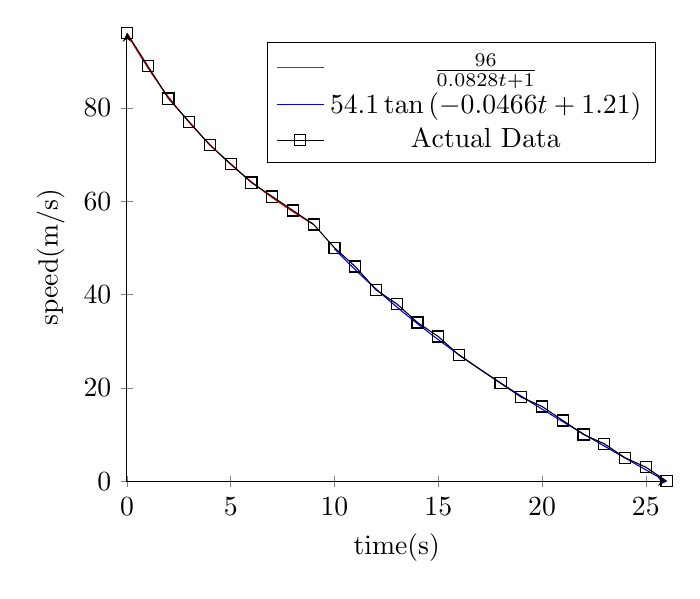
\begin{tikzpicture}
\begin{axis}[
    axis lines = left,
    xlabel = time(s),
    ylabel = speed(m/s),
]
%Below the red parabola is defined
\addplot [
    domain=0:9,
    samples=100, 
    color=red,
]
{96/(0.0828*x + 1)};
\addlegendentry{$\frac{96}{0.0828t + 1}$}
%Here the blue parabloa is defined
\addplot [
    domain=10:26, 
    samples=100, 
    color=blue,
    ]
    {54.1*(tan((-0.0466*x + 1.21)*(180/3.1415)))};
\addlegendentry{$54.1\tan{(-0.0466t+1.21)}$}

 \addplot[
    color=black,
    mark=square]
    coordinates {(0,96)(1,89)(2,82)(3,77)(4,72)(5,68)(6,64)(7,61)(8,58)(9,55)(10,50)(11,46)(12,41)(13,38)(14,34)(15,31)(16,27)(18,21)(19,18)(20,16)(21,13)(22,10)(23,8)(24,5)(25,3)(26,0)};
\addlegendentry{Actual Data}
\end{axis}
\end{tikzpicture}
\caption{Graph of model 3, when $m=125,000kg$}
\end{figure}

From this graph, we can clearly see that there is not much of a difference by taking $m=125000kg$. The difference is also very hard to see and taking $m=125,000kg$, doesn't have much of a difference on the model and the RMS error also works out to be 0.17. This means that not much has changed and that the model still very well models the landing of the aeroplane.
\subsection{Considering effect on model is mass is $m=115000kg$}

\subsubsection{Solutions of the DE}
\textbf{Case1: }
Using the equation from 4.2 for case 1, we see that:
\begin{align*}
    v &= \frac{m}{c_{1}m+kt}
\end{align*}

Then using the point (t=0, v=96), we see that:
\begin{center}
\begin{align*}
    v &= \frac{m}{kt+cm}
    \\ 96 &= \frac{1}{c_1}
    \\ c &= \frac{1}{96}
\end{align*}
\end{center}
Using the point (t=9, v=55), we see that:
\begin{center}
\begin{align*}
    v &= \frac{m}{kt+c_1m}
    \\ 55 &= \frac{m}{9k + c_1m} = \frac{96m}{864k + m} && \text{As $c=\frac{1}{96}$}
    \\ 864k &= \frac{96}{55}m - m
    \\ k &= \frac{1}{864}(\frac{96}{55}m - m)
    \\ &= \text{99.22 $N/ms^{-1}$}
\end{align*}
\end{center}
From this we can deduce that for case 1, if $m=115000kg$:
\begin{center}
\begin{align*}
    v &= \frac{m}{kt+c_{1}m}
    \\ v &= \frac{1}{\frac{k}{m}t+\frac{1}{96}}
    \\ \Aboxed{v &= \frac{96}{0.08283t + 1}}
\end{align*}
\end{center}

\textbf{Case 2: } 
Using the equation from 4.2 for case 2, we see that:

\begin{align*}
    \sqrt{\frac{k}{F_b}} \arctan{(v\sqrt{\frac{k}{F_b}})} &= -\frac{k}{m}t + c_2
\end{align*}
Then using the point (t=26, v=0), we see that:
\begin{center}
\begin{align*}
    \sqrt{\frac{k}{F_b}} \arctan{(v\sqrt{\frac{k}{F_b}})} &= -\frac{k}{m}t + c_2
    \\ -\frac{26k}{m} + c_2 &= 0
    \\ c_2 &= \frac{26k}{m} 
    \\ &= 0.02243
\end{align*}
\end{center}
This means our equation now becomes:
\begin{equation}
    \sqrt{\frac{k}{F_b}} \arctan{(v\sqrt{\frac{k}{F_b}})} = -\frac{k}{m}t + 0.02243
\end{equation}
\\ \\
After this using the point (t=9, v=55), we see that:
\\
\begin{center}
\begin{align*}
    \sqrt{\frac{k}{F_b}} \arctan{(v\sqrt{\frac{k}{F_b}})} &= -\frac{k}{m}t + 0.02243
    \\ \sqrt{\frac{k}{F_b}} \arctan{(55\sqrt{\frac{k}{F_b}})} &= -9\frac{k}{m} + 0.02243
\end{align*}
\end{center}
To find $F_b$, we can use Newton-Raphson, by letting $\alpha=\sqrt{\frac{k}{F_b}}$ and substituting $9 \frac{k}{m} = 7.765\times{10^{-3}}$
\begin{align*}
    \alpha \arctan{(55\alpha)} &= -9 \frac{k}{m} + 0.02243
\end{align*}
\begin{equation}
    \alpha \arctan{(55\alpha)} - 0.01466 = 0
\end{equation}
Thus by applying Newton-raphson on the above equation, we will be able to find alpha, giving us a value for $F_b$

\subsubsection{Using Newton-Raphson to find $\alpha$}
\begin{align*}
    \text{let } f(\alpha) &= \alpha \arctan{(55\alpha)} - 0.01466
    \\ \text{Therefore } f'(\alpha) &= \arctan{55a} + \frac{55\alpha}{1+3025\alpha^2}
\end{align*}

\begin{figure}[H]
\centering

\begin{tikzpicture}
\begin{axis}[
    %axis lines = left,
    xlabel = x,
    ylabel = $f(x)$,
]
%Below the red parabola is defined
\addplot [
    domain=0:0.02,
    samples=100, 
    color=red,
]{x*rad(atan(55*x))-0.01466};
\addlegendentry{$xatan{55x}-0.01466$}
\end{axis}
\end{tikzpicture}
\caption{Graph showing the graph of $f(x)$}
\end{figure}

Using the graph of $f(x)$, we see that the root is close to 0.02. Therefore we will use 0.02 as our initial guess for the root.
\\ \\
Using the iterative formula, $x_{i+1} := x_{i}-\frac{f(x)}{f'(x)}$, to find the next closest root we can produce a table showing all the iterations and the next approximation of the root it gave.

\begin{table}[h]
\centering
    \begin{tabular}{|l|l|l|l|l|}
        \hline
        i & $x_i$ & $f(x)$ & $f'(x)$ & $x_{i+1}$ \\ \cline{1-5}
        1 & 0.02000 & 0.00200 & 1.3307 & 0.01850 \\ \cline{1-5}
        2 & 0.01850 & 0.00003 & 1.2939 & 0.01848 \\ \cline{1-5}
        3 & 0.01848 & 0.00000 & 1.2933 & 0.01848 \\ \cline{1-5}
    \end{tabular}
    \caption{Newton-Raphson Iterations}
\end{table}
\
Thus we find that alpha is 0.01848, meaning that the fraction \\ $\sqrt{\frac{k}{F_b}} = 0.01848$ to 5dp.
\newline \newline
Therefore by rearranging for v, we can conclude that for case 2, when $m=115000kg$:
\begin{align*}
    \alpha \arctan{(\alpha v)} &= -\frac{k}{m}t + 0.02243
    \\ \arctan{(\alpha v)} &= -\frac{k}{m\alpha}t + \frac{0.02243}{\alpha}
    \\ v &= \frac{1}{\alpha} \tan{(-\frac{k}{m\alpha}t + \frac{0.02243}{\alpha})}
    \\ \Aboxed{v &=  54.1\tan{(-0.0467t + 1.21)}}
\end{align*}

\input{Model3/ParameterVariation/LowerBoundComparison.tex}